\documentclass{article}

\usepackage{graphicx}
\usepackage{tikz}
\usepackage{tikzsymbols}
\usetikzlibrary{calc,patterns,shapes.geometric}
\pagestyle{empty}
\usepackage[margin=0pt]{geometry}
\geometry{papersize={14in,12in}}

\def\centerarc[#1](#2)(#3:#4:#5){\draw[#1] ($(#2)+({#5*cos(#3)},{#5*sin(#3)})$) arc (#3:#4:#5);}

\begin{document}
	\begin{figure}
		\centering
		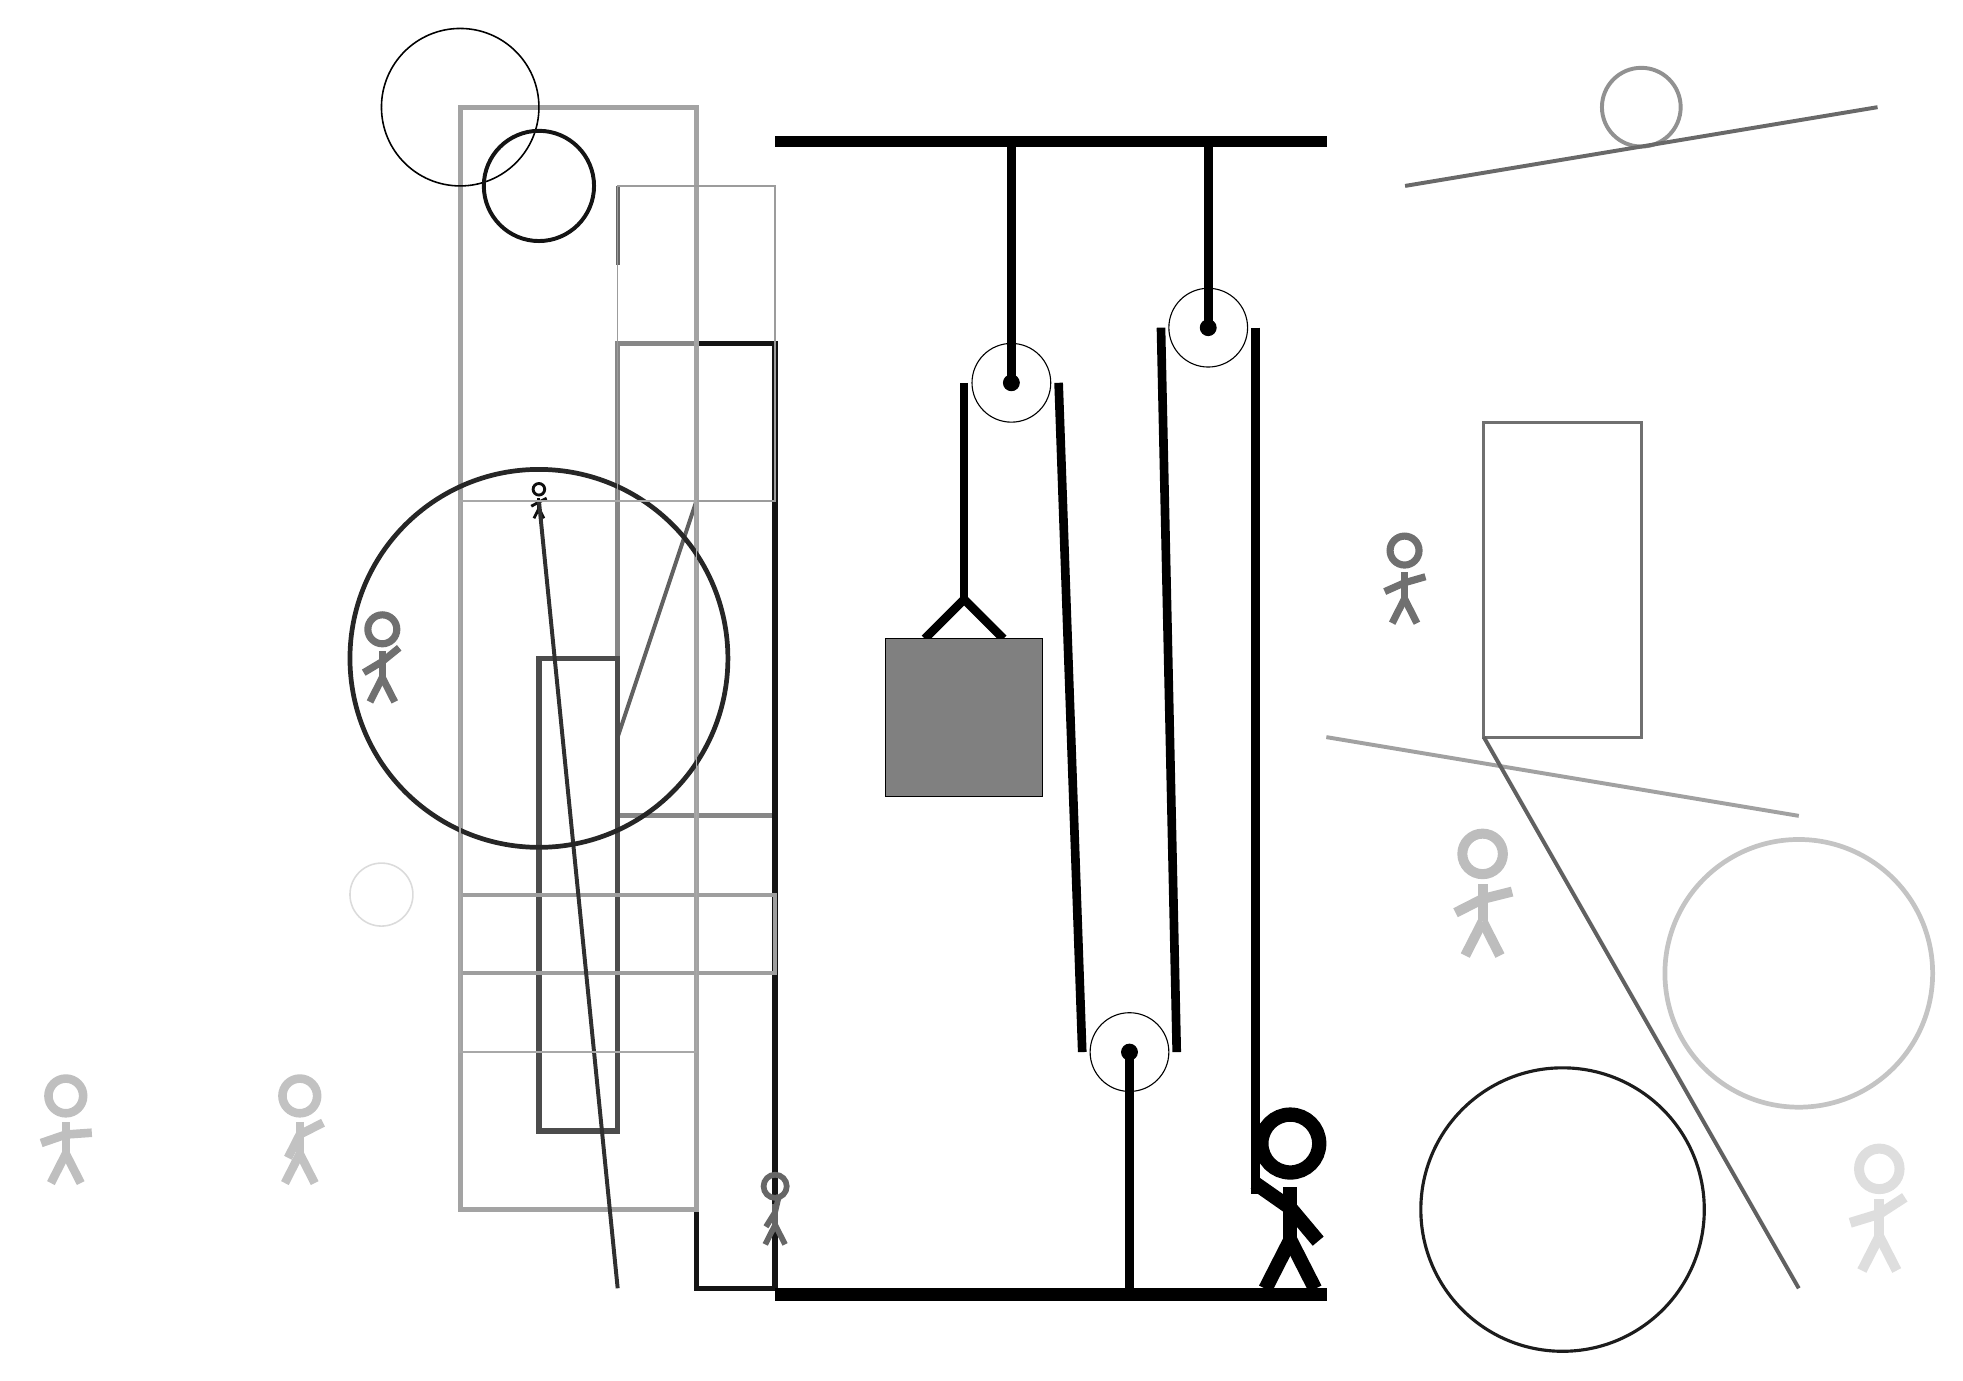
\begin{tikzpicture}
			%%%%% START %%%%%
			
			\draw[fill=black] (-2, 11.5) rectangle (5, 11.625);
			
			\draw (1, 8.5) circle (0.5);
			\draw[fill=black] (1, 8.5) circle (0.1);
			\draw[line width=1.1mm]  (1, 11.5) -- (1, 8.5);
			
			\draw[fill=white](2.5, 0.0) circle (0.5);
			\draw[fill=black] (2.5, 0.0) circle (0.1);
			\draw[line width=1.1mm]  (2.5, -3) -- (2.5, 0.0);
			
			\draw[line width=0.6mm, color=black!47] (-4, 9) rectangle (-2, 3);
			
			\draw[line width=0.5mm, color=black!37](5, 4) -- (11, 3);
			\draw[line width=0.5mm, color=black!62](-4, 4) -- (-3, 7);
			\draw[line width=0.7mm, color=black!70] (-4, -1) rectangle (-5, 5);
			\node[line width=0.7mm, color=black!94] at (-5, 7) {\Strichmaxerl[2][28][27]};
			
			\draw[line width=0.7mm, color=black!92] (-3, 9) rectangle (-2, -3);
			\draw [line width=0.4mm, color=black!89](8, -2) circle (1.8);
			
			\draw[line width=0.5mm, color=black!38] (-2, 1) rectangle (-6, 2);
			\node[line width=0.3mm, color=black!13] at (12, -2) {\Strichmaxerl[7][17][33]};
			
			\node[line width=0.7mm, color=black!26] at (7, 2) {\Strichmaxerl[7][27][14]};
			\draw[line width=0.6mm, color=black!36] (-3, -2) rectangle (-6, 12);
			\draw[line width=0.5mm, color=black!60](-4, 10) -- (-4, 11);
			\node[line width=0.4mm, color=black!56] at (-7, 5) {\Strichmaxerl[5][31][39]};
			\node[line width=0.4mm, color=black!25] at (-11, -1) {\Strichmaxerl[6][19][4]};
			\draw [line width=0.6mm, color=black!90](-8, 0) circle (0.0);
			\draw[line width=0.5mm, color=black!81](-4, -3) -- (-5, 7);
			
			\draw [line width=0.6mm, color=black!23](11, 1) circle (1.7);
			
			\draw [line width=0.5mm, color=black!43](9, 12) circle (0.5);
			\draw [line width=0.6mm, color=black!85](-5, 5) circle (2.4);
			\node[line width=0.3mm, color=black!56] at (6, 6) {\Strichmaxerl[5][24][16]};
			\draw[line width=0.2mm, color=black!39] (-4, 11) rectangle (-2, 7);
			
			\draw[line width=0.2mm, color=black!34] (-3, 0) rectangle (-6, 7);
			\node[line width=0.7mm, color=black!24] at (-8, -1) {\Strichmaxerl[6][63][27]};
			\draw [line width=0.2mm, color=black!100](-6, 12) circle (1.0);
			\draw[line width=0.5mm, color=black!59](6, 11) -- (12, 12);
			
			\node[line width=0.4mm, color=black!60] at (-2, -2) {\Strichmaxerl[4][58][77]};
			\draw [line width=0.2mm, color=black!14](-7, 2) circle (0.4);
			\draw [line width=0.5mm, color=black!92](-5, 11) circle (0.7);
			\draw[line width=0.4mm, color=black!56] (7, 8) rectangle (9, 4);
			\draw[line width=0.5mm, color=black!62](7, 4) -- (11, -3);
			
			\draw[fill=white](3.5, 9.2) circle (0.5);
			\draw[fill=black] (3.5, 9.2) circle (0.1);
			\draw[line width=1.1mm] (3.5, 11.5) -- (3.5, 9.2);
			
			\draw[line width=1.1mm] (-0.1, 5.25) -- (0.4, 5.75) -- (0.9, 5.25);
			\draw[fill=black!50] (-0.6, 5.25) rectangle (1.4, 3.25);
			
			\draw[line width=1.1mm] (0.4, 8.5) -- (0.4, 5.75);
			\centerarc[line width=1.1mm](1, 8.5)(0:180:0.6);
			\draw[line width=1.1mm](1.6, 8.5) -- (1.9, 0.0);
			\centerarc[line width=1.1mm](2.5, 0.0)(180:360:0.6);
			\draw[line width=1.1mm](3.1, 0.0) -- (2.9, 9.2);
			\centerarc[line width=1.1mm](3.5, 9.2)(0:180:0.6);
			\draw[line width=1.1mm](4.1, 9.2) -- (4.1, -1.8);
			
			\node at (4.5, -1.9) {\Strichmaxerl[10][-35][-50]};
			
			\draw[fill=black] (-2, -3) rectangle (5, -3.15);
			
			%%%%% END %%%%%
		\end{tikzpicture}
	\end{figure}	
\end{document}